\chapter{Projekcije in zmanjšanje dimenzionalnosti podatkov}

Modeli, ki jih gradimo v strojnem učenju, povzemajo podatke tako, da v nekem formalnem zapisu predstavijo glavne vzorce, ki so te podatke oblikovali. V primeru večdimenzionalnih podatkov nas tako na primer zanima, ali bi podatke lahko popisali z manjšim številom spremenljivk. Z izborom značilk smo se ukvarjali že v prejšnjem poglavju, a nas bo tu zanimalo, če lahko podatke predstavimo z novimi značilkami, ki bi podatke lahko predstavili bolj kompaktno, pri tem odkrili kakšno zanimivo preslikavo starih v nove značilke, ter morda celo dosegli, da je novih značilk izjemno malo. Recimo, dve, tako da lahko vse primere izrišemo v razsevnem diagramu in tam s pomočjo vizualizacije razmišljamo o njihovih podobnosti in strukturi prostora primerov. Ljudje smo vizualna bitja in nam izris kart primerov lahko intuitivno pove več kot pa recimo matematične enačbe, ki morda te povezujejo.

Začnimo s primerom. Na sliki~\ref{f:torbice} so ženske torbice različnih proizvajalcev. Z uporabo že zgrajenih globokih mrež za razvrščanje slik lahko slike torbic pretvorimo v vektorje. Mreža Inception v3 nam na svojem predzadnjem nivoju na primer za vsako sliko vrne vektor dolžine 2048, oziroma sliko popiše z 2048 atributi. S postopki, ki jih bomo opisali v tem poglavju, lahko take opise zmanjšamo in predstavimo torbice v nizko dimenzionalnem prostoru. Slika~\ref{f:torbice-mds} tako prikazuje predstavitev primerov v dvodimenzionalnem prostoru, kjer je razvidno, da ena Hermesova torbica bolj podobna torbicam ostalih proizvajalcev, in da se je Dior pri eni od torbic zgledoval po torbicah Chanela. Morda. Vsekakor bi ta opažanja morali preveriti, a je zanimivo, kako hitro nas vizualizacije navdahnejo z idejami. Prav zato so vizualizacije v odkrivanju znanj iz podatkov tako pomembne in zato so pomembne tudi tehnike zmanjšanja dimenzionalnosti in odkrivanja nizko dimenzionalnih projekcij podatkov.

\begin{figure}[htbp]
\centering{
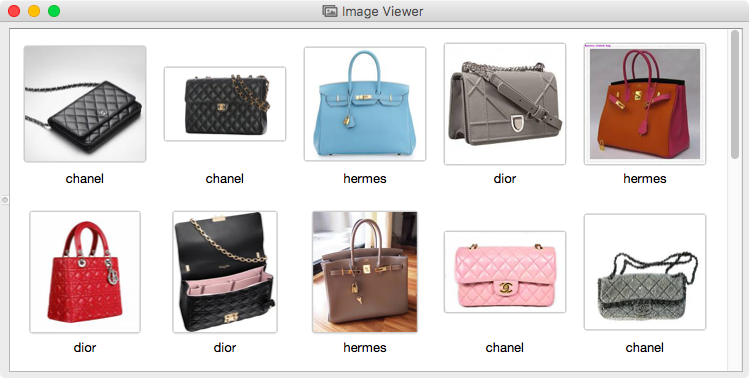
\includegraphics[width=12cm]{slike/torbice.png}
\caption{Ženske torbice različnih proizvajalcev.}
\label{f:torbice}}
\end{figure}

\begin{figure}[htbp]
\centering{
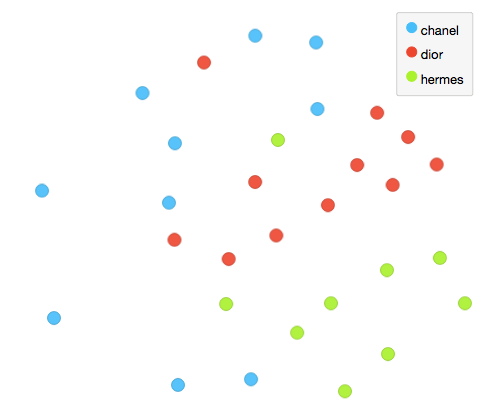
\includegraphics[width=8cm]{slike/torbice-mds.png}
\caption{Predstavitev ženskih torbic s slike~\ref{f:torbice} v dvodimenzionalnem prostoru.}
\label{f:torbice-mds}}
\end{figure}

\section{Metoda glavnih komponent}

Prva, morda tudi najbolj znana metoda za zmanjšanje dimenzij in odkrivanje zanimivih projekcij podatkov je metoda glavnih komponent. Predpostavimo, da imamo dano matriko učnih primerov $X\in\mathbb{R}^{m\times n}$, kjer je $m$ število primerov in $n$ število atributov. Primer $x^{(i)}\in X$, torej $i$-ti primer v učni množici primerov, bo tako opisan z $n$ atributi $x\in\mathbb{R}^{n}$, za katere bomo tu privzeli, da so njihove vrednosti realna števila. V splošnem iščemo projekcije podatkov tako, da atributni zapis primerov z $n$ atributi nadomestimo z atributnim zapisom z $k$ novimi atributi tako, da je $k\ll n$ in da nam novi atributi povedo čim več o primerih iz učne množice.

Pričnimo s $k=1$, torej s projekcijo v eno samo dimenzijo. Dogovorimo se, da bo naša projekcija linearna in da bomo vrednost novega atributa tvorili kot linearno kombinacijo originalnih atributov. Smer projekcijske ravnine oziroma smer premice, na katero bomo projicirali podatke označimo z enotskim vektorjem $u_1$, za katerega torej velja $u_1^\tr u_1=1$.

Naj bo $x^{(i)}$ primer iz učne množice. Njegova projekcija na projekcijsko ravnino je skalar, $u_1 x^{(i)}\in \mathbb{R}$. Naj bo $\bar{x}$ središčna točka podatkov:
%
$$ \mean{x}=\frac{1}{m}\sum_i x^{(i)}$$
%
Projekcija središčne točke na projekcijsko ravnino je $u_1 \mean{x}$. Primeri v učni množici odstopajo od središčne točke, eni bolj, drugi manj. Primere bi želeli projicirati na ravnino tako, da ta odstopanja čim bolj zajamemo, torej, da so tudi v projicirani ravnini čim večja. Povprečno kvadratno odstopanje v projekciji od projekcije središčne točke imenujemo tudi varianca točk v projekciji:
%
$$ \Var(u_1^\tr X^\tr)=\frac{1}{m}\sum_{i=1}^m \big(u_1^\tr x^{(i)}-u_1^\tr\mean{x}\big)^2 $$

Z drugimi besedami, želimo poiskati tak projekcijski vektor $u_1$, ki maksimizira varianco projekcije $\Var(u_1^\tr X^\tr)$. Poigrajmo se malce z enačbo za varianco projekcije:
%
\begin{equation}
  \begin{split}
    \Var(u_1^\tr X^\tr)
    & = \frac{1}{m}\sum_{i=1}^m \big(u_1^\tr x^{(i)}-u_1^\tr\mean{x}\big)^2 \\
    & = \frac{1}{m}\sum_{i=1}^m \big(u_1^\tr x^{(i)} u_1^\tr x^{(i)} - 2 u_1^\tr x^{(i)} u_1^\tr \mean{x} + u_1^\tr \mean{x} u_1^\tr \mean{x} \big)
  \end{split}
\end{equation}
%
Tu upoštevamo, da je $u_1^\tr x$ skalarni produkt dveh vektorjev, in da je transponirana vrednost realnega števila enaka temu številu. Torej je na primer $u_1^\tr x=(u_1^\tr x)^\tr=x^\tr u_1$. Z upoštevanjem tega se nam zgornji izraz primerno poenostavi:
%
\begin{equation}
  \begin{split}
    \Var(u_1^\intercal X^\tr)
    & = \frac{1}{m}\sum_{i=1}^m u_1^\tr \big(x^{(i)} {x^{(i)}}^\tr - 2 x^{(i)} \mean{x}^\tr + \mean{x}~\mean{x}^\tr \big) u_1 \\
    & = u_1^\tr \big( \frac{1}{m}\sum_{i=1}^m (x^{(i)}-\mean{x}) (x^{(i)}-\mean{x})^\tr\big) u_1
  \end{split}
\end{equation}

V oklepaju je kovariančna matrika! Prejšnji stavek smo končali s klicajem zato, ker je kovarianca znan in mnogokrat uporabljan koncept v statistiki in nam pove, kako sta dve naključni spremenljivki povezani. Označimo kovariančno matriko s ${\rm S}$:
\begin{equation}
  {\rm S} = \frac{1}{m}\sum_{i=1}^m (x^{(i)}-\mean{x}) (x^{(i)}-\mean{x})^\tr
\end{equation}

V našem primeru imamo $n$ atributov, kar pomeni, da je kovariančna matrika dimenzije ${\rm S}=\mathbb{R}^{n\times n}$. Zapišimo še enkrat dobljeno enačbo za varianco:
\begin{equation}
  \Var(u_1^\intercal X^\tr) = u_1^\tr {\rm S} u_1
\end{equation}
%
Spomnimo, da je naš namen poiskati projekcijski vektor $u_1$ pri katerem je zgornja varianca maksimalna. Za vektor $u_1$ zahtevamo, da je to enotni vektor (sicer maksimizacija zgornje enačbe ne bi imela smisla, saj bi to dosegli z neskončno dolgim vektorjem $u_1$). Maksimizacijo variance, kjer iščemo ustrezen vektor $u_1$ z omejitvijo $u_1^\tr u_1=1$ rešimo z uporabimo Lagrangeovih multiplikatorjev. Maksimiziramo torej izraz:
%
\begin{equation}
  f(u_1) = u_1^\tr {\rm S} u_1 + \lambda_1(1-u_1^\tr u_1)
\end{equation}
%
V maksimumu bo odvod zgornje enačbe enak nič:
\begin{equation}
  \frac{\partial f(u_1)}{\partial u_1}={\rm S} u_1 - \lambda_1 u_1=0
\end{equation}
%
kar pomeni,
\begin{equation}
  {\rm S} u_1=\lambda_1 u_1
\end{equation}
%
Tu je ${\rm S}$ matrika katere vrednosti poznamo, $u_1$ je vektor, ki ga iščemo, $\lambda_1$ pa skalar. Poznano? Seveda! Zgornjemu pogoju ustreza le tak $u_1$, ki je lastni vektor matrike ${\rm S}$. Ampak korelacijska matrika ima več lastnih vektorjev. Kateri med njimi je pravi? Množimo zgornjo enačbo z $u_1^\tr$:
%
\begin{equation}
  u_1^\tr {\rm S} u_1 = u_1^\tr \lambda_1 u_1=\lambda_1 u_1^\tr u_1=\lambda_1
\end{equation}
%
Na levi je izraz za našo varianco $\Var(u_1^\intercal X^\tr)$, ki jo skušamo maksimizirati. Vemo, da mora biti $u_1$ lastni vektor kovariančne matrike. Skladno z zgornjo enačbo pa sedaj tudi vemo, da je to lastni vektor z najvišjo pripadajočo lastno vrednostjo.

V smeri vektorja $u_1$ se lega naših primerov $X$ v $n$-dimenzionalnem prostoru torej najbolj spreminja, njihova varianca je v tej smeri največja. Z $u_1^\tr X^\tr$ dobimo pravokotno projekcijo vsakega od primerov na to os. S to projekcijo, oziroma legi v smeri $u_1$, smo pojasnili največjo varianco primerov. Kaj še ostane? Vse, kar je pravokotno na smer $u_1$. Največjo varianco na pravokotni hiperravnini pa je ravno v smeri drugega lastnega vektorja, saj je ta pravokoten na $u_1$, to je vektorja, ki ima drugo največjo lastno vrednost. Pojasnjen delež te variance je $\lambda_2$, skupaj pa s pravokotno projekcijo na prvi in drugi lastni vektor pojasnimo $\lambda_1+\lambda_2$ variance množice primerov.

Lastni vektorji kovariančne matrike nam določajo nov koordinatni
sistem, kjer so koordinate, po vrsti, tiste, po katerih se lege točk v
večdimenzionalnem prostoru najbolj spreminjajo, oziroma je njihova
varianca največja. Nove koordinate, urejene skladno z lastnimi vrednostmi vektorjev, imenujemo komponente primerov v novem, transformiranem sistemu. Ker nas bodo zanimale samo te z visokimi deleži razložene variance jih bomo imenovali {\em glavne komponente}.

\begin{figure}[htbp]
\centering{
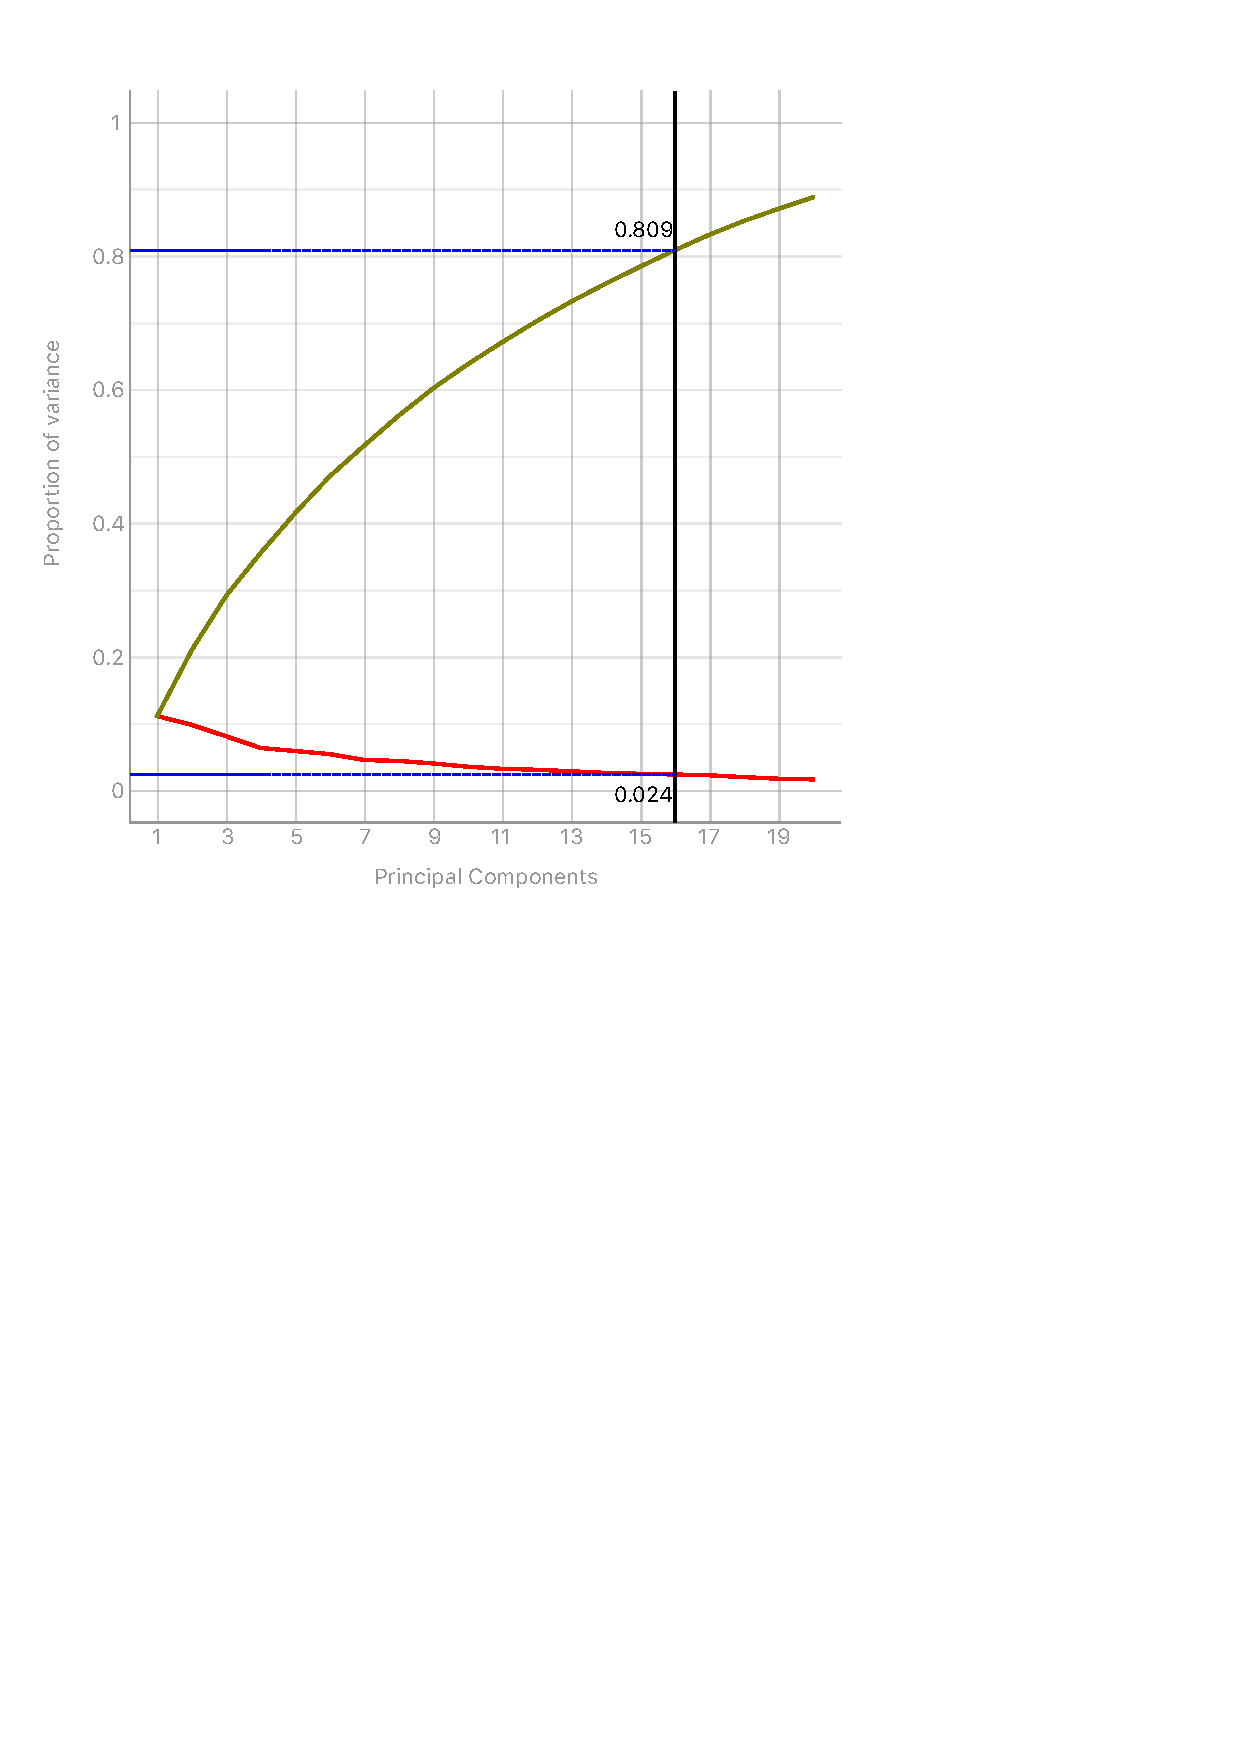
\includegraphics[width=8cm]{slike/scree-diagram.pdf}
\caption{Graf odvisnosti razložene variance od števila glavnih komponent (zgornja črta) za podatke o torbicah iz slike~\ref{f:torbice}.}
\label{f:scree}}
\end{figure}

V splošnem nas zanima, koliko najvišje rangiranih dimenzij v novem
koordinatnem sistemu zares potrebujemo za opis podatkov. Pri tem moramo
seveda določiti, kakšen je naš ciljni delež pojasnjene variance. Tipično
smo zadovoljni, če izbrano število komponent pojasni vsaj $80\%$ skupne variance. Ker skupno varianco poznamo (enaka je vsoti kvadratov razdalj do
centra), je potrebno torej le določiti, koliko začetnih urejenih lastnih
vrednosti moramo sešteti, da njihova vsota predstavlja želeni delež razložene variance. Primer grafa, ki kaže odvisno deleža razložene variance glede na število glavnih komponent kaže slika~\ref{f:scree}.

Pristop glavnih komponent se mnogokrat uporablja tudi samo za namene vizualizacije, kjer primere, opisane z mnogimi atributi, želimo predstaviti v dvodimenzionalni ravnini. Pri tem se moramo seveda zavedati, da prvi dve komponenti razložijo morda le majhen del celotne variance.

Za predstavitev podatkov z glavnimi komponentami je potrebno podatke najprej osrediščiti in nato poiskati kovariančno matriko. Lastni vektorji kovariančne matrike so bazni vektorji novega, transformiranega sistema, njihove lastne vrednosti pa povedo, kakšen delež variance nam razloži posamezna komponenta.

Še praktičen razmislek: v primerih velikega števila atributov bo računanje vseh lastnih vektorjev in vrednosti zamudno. Še posebej, če nas zanima samo projekcija podatkov v dvodimenzionalni prostor. Prvi lastni vektor kovariančne matrike $M$ lahko rajši (hitreje) določimo numerično, s potenčno metodo. Vzamemo nek naključni vektor (npr. $x$), ga transformiramo z matriko $M$ (torej, izračunamo $x\leftarrow M x$), in to ponavljamo do konvergence. Ob vsakem koraku tako dobljeni $x$ normaliziramo, torej, $x\leftarrow \frac{M x}{\norm{M x}}$. Na ta način dobimo lastni vektor. Kako izračunamo pripadajočo lastno vrednost?
\begin{equation}
  M u = \lambda u
\end{equation}

\begin{equation}
  u^\tr M u = u^\tr \lambda u = \lambda u^\tr u = \lambda
\end{equation}

Kako določimo naslednjo komponento? Ena od možnosti je, da uporabimo ravnokar izračunani lastni vektor, nanj projiciramo podatke, te vrednosti odštejemo od podatkov (torej dobimo projekcijo na lastnemu vektorju pravokotno hiperravnino) in za te podatke ponovno izračunamo kovariančno matriko ter s potenčno metodo njej lastni vektor z največjo lastno vrednostjo. V primeru, da potrebujemo več komponent, postopek ustrezno ponovimo.

Za primer, ko nas zanima samo projekcija podatkov v ravnino lahko potenčno metodo namesto na vektorju izvedemo na sistemu dveh vektorjev $U$. Vektorja matrike $U$ morata biti pravokotna. To dosežemo tako, da po vsakem koraku potenčne metode uporabimo Gram-Schmidtovo ortogonalizacijo.

\section{Večrazredno lestvičenje}

Pri zmanjšanju dimenzij nam je lahko cilj, da ohranimo razdalje med posameznimi primeri. Tu predpostavimo, da za vsak par primerov znamo med njimi oceniti razdaljo. Se pravi, če imamo primere predstavljene v atributnem zapisu, potem uporabimo recimo Evklidsko razdaljo ali pa kosinusno podobnost. Lepota tehnike, ki jo bomo predstavili v tem razdelku je, da nas ne zanima, kako je bila podobnost oziroma razdalja med primeri ocenjena. Lahko smo na vhodu na primer imeli tekstovne dokumente, za katere razdaljo recimo izračunamo s kakšno kompresijsko tehniko. Ali pa filme, za katere razdaljo izračunamo z ozirom na njihovo gledanost v spletni sposojevalnici. Ali pa čivke, ki jih primerjamo med sabo glede na to, kdo jih je všečkal.

Naj bo razdalja med primeroma enaka $\delta_{ij}$. Sedaj te primeri vložimo, recimo, v dvodimenzionalno projekcijo tako da vsakemu primeru $i$ pripišemo koordinati $\vect{\theta}^{(i)}=(\theta_1^{(i)},\theta_2^{(i)})$. Želeli bi, da se v njej razdalje ohranjajo, to je, da je projekcijska razdalja, ki naj bo $d_{ij}$, čimbolj podobna originalni razdalji med primeroma. Razdalja primerov v projekcijskem prostoru je:
$$\delta_{ij}=\norm{{\vect{\theta}}^{(i)}-\vect{\theta}^{(j)}}$$

Računalniška izvedba algoritma, ki poišče tako vložitev, imenujemo večrazsežnostno lestvičenje ({\em multidimensional scaling}, MDS). Formalno ciljno funkcijo problema zastavimo tako, da določimo energijo sistema ali napetost ({\em stress}) kot, recimo,
$$J(\mathbf{X}) = \sum_{i\ne j} (d_{ij} - \delta_{ij})^2,$$
kjer je $\mathbf{X}$ trenutni razpored točk, $d_{ij}$ in $\delta_{ij}$ pa trenutna projekcijska in želena razdalja med primeroma $i$ in $j$. Večrazsežnostno lestvičenje poišče razpored $\mathbf{X}$ z najmanjšo napetostjo $J(\mathbf{X})$ oziroma najmanjšo vrednostjo kriterijske funkcije.

Kako minimizirati takšno funkcijo? Analitično ne bo šlo. Za to bi bilo potrebno odvesti $\sigma(\mathbf{X})$ po vseh koordinatah $\theta_1^{(i)}$ in $\theta_2^{(i)}$ in poiskati ničle:
\begin{eqnarray}
  \frac{\partial\sigma({\mathbf{X}})}{\partial \vect{\theta_k}} & = &
  \sum_{j\ne i} \frac{\partial\sigma({\mathbf{X}})}{\partial d_{ij}}\frac{d_{ij}}{\partial \vect{\theta_k}} \nonumber \\
  & = & - \sum_{j\ne i} 2\left(\sqrt{(\theta_1^{(i)}-\theta_1^{(j)})^2+(\theta_2^{(i)}-\theta_2^{(j)})^2}-\delta_{ij}\right) \frac{(\theta_k^{(i)}-\theta_k^{(j)})}{\sqrt{(\theta_1^{(i)}-\theta_1^{(j)})^2+(\theta2^{(i)}-\theta_2^{(j)})^2}} \nonumber \\
& = & - \sum_{j\ne i} 2\left(d_{ij}-\delta_{ij}\right) \frac{(\theta_k^{(i)}-\theta_k^{(j)})}{d_{ij}} \label{eq:mds-grad}
\end{eqnarray}
Pri stotih točkah bi dobili sistem z dvesto takšnimi enačbami; ideji o direktnem napadu se torej raje odpovemo.

Drug, izvedljiv postopek je gradientna metoda: kot pri dosedanjih pristopih z gradientnim spustom (recimo, linearna regresija) izračunamo gradient funkcije kriterijske funkcije $J(\mathbf{X})$. To smo pravzaprav storili že zgoraj. Izberemo si poljuben začetni razpored točk, vstavimo koordinate v odvode, dobimo gradient (vektor odvodov) in se pomaknemo v smeri nasprotni gradientu, se pravi, vse točke pomaknemo v smer, kamor jih potiskajo odvodi. Gradientna metoda bi delovala, vendar ne prav dobro. Bila bi počasna in velikokrat bi nas (lahko) pripeljala le v lokalni minimum.

V svetu optimizacijskih problemov je gradientna metoda le metoda grobe sile, ki jo bomo uporabili, če se ne moremo spomniti ničesar boljšega. Eden od boljših postopkov je ``majorizacija''. Označimo funkcijo, katere minimum iščemo, z $f(x)$. Recimo, da si znamo izmisliti, neko drugo funkcijo $g(x, y)$, ki je stalno večja ali enaka $f(x)$ (torej, za vsak $y$ velja $g(x, y)\ge f(x)$ pri vsakem $x$), v točki $g(x, x)$ pa velja $g(x, x)=f(x)$. Funkcija $g(x, y)$ naj bo takšna, da znamo dobro poiskati vrednost $x$, pri katere doseže minimum. Zdaj lahko počnemo tole: izmislimo si začetni $x_0$. Pri njem, vemo, velja $g(x_0, x_0)=f(x_0)$. Minimiziramo funkcijo $g$ in dobimo nov, boljši $x$ - označimo ga z $x_1$. Vrednost $g(x_1, x_0)$ je manjša ali enaka vrednosti $g(x_0, x_0)$, saj smo minimizirali $g$ po prvem argumentu. Po drugi strani, spet po definiciji funkcije $g$, velja $f(x_1) \le g(x_1, x_0)$. Imamo torej
$$f(x_1) \le g(x_1, x_0) \le g(x_0, x_0) = f(x_0)$$
Postopek ponovimo z $x_1$, da pridelamo naslednji, še boljši $x_2$.

Takšna optimizacija je, tako kot gradientna metoda še vedno iterativna, vendar hitrejša. Koliko hitrejša, je odvisno od tega, kako dobro $g(x, y)$ smo poiskali; $g(x, y)$ se mora čim tesneje prilegati $f(x)$, poleg tega pa jo moramo biti zmožni čim boljše optimizirati.

Algoritem večdimenzionalnega lestvičenja, ki deluje na ta način, se imenuje SMACOF \angl{scaling by majorizing a complicated function}. SMACOF je hitrejši od gradientne metode, dela večje korake in se manjkrat zatakne v lokalnih ekstremih, zato je uporabnejši za (realistične) primere, v katerih je točk veliko.

Za izračun napetosti lahko namesto gornje, naivne formule uporabljamo tudi takšne, ki uteži prispevke parov (predpišemo lahko, za katere pare si še posebej želimo, da bi razdalja ustrezala pravi), poleg tega pa lahko napetost posameznega para normiramo tako, da jo delimo z želeno ali s trenutno razdaljo.

Slika~\ref{f-zoo-mds} kaže zemljevid živali. Razdalje med pari živali so izračunane kot evklidske razdalje med atributi, ki jih opisujejo. Točke, ki predstavljajo živali, smo obarvali glede na vrsto -- vijolični so sesalci, rdeče ptice, oranžno žuželke. Povezani so pari živali, ki so si med seboj najbolj podobne.

\begin{figure}[tbp]
\begin{center}
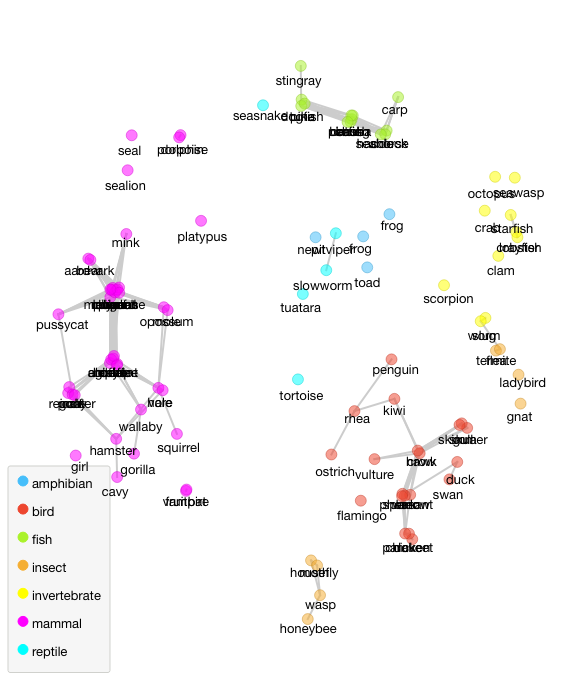
\includegraphics[width=10cm]{slike/zoo-mds.png}
\caption{Zemljevid živali (podatkovna zbirka Zoo). Vrsta živali je označena z barvo. Nekatere oznake so zaradi prekrivanj neberljive in bi razvojnike programa potrebno opozoriti, da v vizualizacijo vključijo optimizacijo postavitve oznak.}
\label{f-zoo-mds}
\end{center}
\end{figure}

Čeprav MDS ni uporabljal podatkov o vrstah živali, so različne vrste na zemljevidu dobro ločene. Vidimo tudi nekaj podobnosti med živalmi: morske sesalce je MDS postavil v bližino rib; dvoživke so blizu rib in nevretenčarjev, predvsem morskih; žuželke so pomešane s ptiči.

Vidimo tudi težavo: žuželke so razdeljene v dve skupini. MDS se je očitno znašel v lokalnem ekstremu, saj bi morale ose in čebele k ostalim žuželkam, vendar bi jih moral optimizacijski postopek peljati okrog ptičev. To se zgodi kar pogosto in pomagamo si tako, da podatke nekoliko potresemo, naključno premaknemo točke, ali pa začnemo celotno optimizacijo znova.

Večrazežnostno lestvičenje je torej postopek, ki vizualizira podatke v obliki zemljevida. Podatki so opisani s seznamom primerov in razdalj med njimi; lastnosti primerov niso potrebne in jih ne znamo upoštevati (razen, če iz le-teh računamo razdalje, kot smo storili pri živalih). Zemljevid je nezanesljiv v tem smislu, da bodo različne naključne začetne postavitve vodile v različne končne slike, a vsaka od njih nam lahko nudi drugačen pogled na podatke. Prav tako je nezanesljiv položaj posameznih točk; dogaja se, da je točka obtičala v lokalnem minimumu, čeprav v resnici ne sodi na to mesto. Takšne točke lahko prepoznamo, če zemljevidu dodamo povezave med najbolj podobnimi pari. Obenem nam takšne povezave pomagajo brati sliko. MDS ne sestavlja gruč, pač pa lahko gruče razberemo sami.

\section{Stohastična vložitev sosedov}

Je lahko še kaj boljšega za vložitev primerov v dvorazsežni prostor kot večrazredno lestvičenje? Oziroma, kaj bi bilo lahko sploh narobe s tehniko MDS? Problem MDS-a je, da se ta osredotoča tako na primere, ki so si v originalnem prostoru blizu, kot tudi na primere, ki so si daleč. MDS skuša ohraniti razdaljo med primeri ne glede na to, kako velika je. Velikokrat pa nas v vizualizacijah zanima samo to, da so primeri, ki so se med seboj podobni, skupaj tudi v projekcijskem prostoru. Torej, ohranjanje razdalje med primere, ki so si med seboj drugačni, nas ne zanima, ali pa nas, recimo, zanima veliko manj kot ohranjanje bližine med seboj podobnih primerov.

Metoda SNE \angl{stochastic neighbor embedding}, ki smo jo tu poslovenili v stohastično vložitev sosedov, temelji na verjetnostni oceni podobnosti dveh primerov. Za primera $i$ in $j$ oziroma njuni vektorski predstavitvi $x^{(i)}$ in $x^{(j)}$ določimo verjetnost $p_{j|i}$, da bi za primer $i$ izbrali soseda $j$, če bi sosede izbirali skladno z Gaussovo verjetnostno porazdelitvijo, ki je centrirana v $x^{(i)}$:
\begin{equation}
  p_{j|i}=\frac{\exp(-\norm{x^{(i)}-x^{(j)}}^2/2\sigma_i^2)}
  {\sum_{k\neq i}\exp(-\norm{x^{(i)}-x^{(k)}}^2/2\sigma_i^2)}
\end{equation}
kjer je $\sigma_i$ varianca Gaussove porazdelitve za točko $i$. Ker nas zanimajo samo modeliranje podobnosti med različnimi točkami, je $p_{i|i}$ enaka nič. Zanima nas vložitev teh primerov v projekcijski prostor, kjer bo lega primerov kot pri MDS določena z vektorji $\vect{\theta}^{(i)}$ in bomo podobno kot zgoraj, le tokrat za projekcijski prostor, sosednost predstavili z verjetnostjo $q_{j_i}$.

Označimo verjetnostne porazdelitve preko vseh sosedov z za primer $i$ in za originalni prostor z $P_i$ in za projekcijski prostor z $Q_i$. Naša želja je, da bi bili ti porazdelitvi med sabo čim bolj podobni. Ker ti dve verjetnostni porazdelitve favorizirajo bližnje primere oziroma so za te verjetnosti visoke, podobnost porazdelitev $P_i$ in $Q_i$ pomeni, da je projekcija ohranila bližnje primere za primer $i$. Mera, ki pove, kako zvesto $q_{j|i}$ sledi $p_{j|i}$ je Kullback-Leibler-jeva divergenca, katere vsoto po primerih želimo minimizirati. Kriterijska funkcija je zato:
\begin{equation}
  J(\vect{\Theta}) = \sum_i KL(P_i\ ||\ Q_i)=\sum_i\sum_j p_{j|i}\log\frac{p_{j|i}}{q_{j|i}}
\end{equation}
Zaradi nesimetričnosti Kullback-Leibler-jeva divergence bodo napake obravnavane nesimetrično: cena za v projekciji oddaljene točke, ki bi sicer morale biti blizu (majhen $q$ in velik $p$) bo večja kot za točke, ki so bližje v projekciji, a bi sicer morale biti daleč (velik $q$ in majhen $p$). Metoda SNE primarno ohranja sosednost.

Med parametri kriterijske funkcije nam je ostal nedoločen še $\sigma_i$, parameter verjetnostne porazdelitve za primer $i$. Metoda SNE ga določi skladno z lokalno gostoto primerov tako, da je za gostejše okolice $\sigma_i$ primerno manjši.

Da bi določili vložitev moramo poiskati lege primerov $\vect{\theta}^{(i)}$ v projekcijskem prostoru. To lahko vnovič storimo z gradientnim sestopom:
%
\begin{equation}
\nonumber
\pd{\vect{\Theta}}{\vect{\theta}^{(i)}}=
  2\sum_j(p_{j|i}-q_{j|i}+p_{i|j}-q_{i|j})(\vect{\theta}^{(i)}-\vect{\theta}^{(j)})
\end{equation}
%
Gradient (popravek) bo večji pri večji razliki med $p$ in $q$ (prvi člen v produktu) med primeroma in bo potekal v smeri vektorja med primeri (drugi člen produkta).

Danes je predvsem znana ``popravljena'' verzija metode SNE, ki jo imenujemo $t$-SNE \angl{t-distributed stochastic neighbor embedding}. V njej Gaussovo porazdelitev za projekcijski prostor zamenjajo s Studentovo $t$-porazdelitvijo, ki ima daljši rep. S to zamenjavo $t$-SNE dovoli, da so primeri, ki so v srednji okolici v originalnem prostoru lahko daleč stran v projekcijski ravnini. Tehnika namesto pogojnih verjetnosti uporablja združene verjetnosti, in simetrično oceno sosednosti za primere v originalnem prostoru,
%
\begin{equation}
  \nonumber
  p_{ij}=\frac{\exp(-\norm{x^{(i)}-x^{(j)}}^2/2\sigma^2)}
  {\sum_{k\neq l}\exp(-\norm{x^{(k)}-x^{(l)}}^2/2\sigma^2)}
\end{equation}
%
ter za projekcijski prostor
\begin{equation}
  \nonumber
  q_{ij}=\frac{(1+\norm{x^{(i)}-x^{(j)}}^2)^{-1}}
  {\sum_{k\neq l}(1+\norm{x^{(k)}-x^{(l)}}^2)^{-1}}
\end{equation}
%
Tudi tu porazdelitvi primerjamo s Kullback-Leiblerjevo divergenco,
\begin{equation}
  \nonumber
  J(\vect{\Theta}) = \sum KL(P\ ||\ Q)=\sum_i\sum_j p_{ij}\log\frac{p_{ij}}{q_{ji}}
\end{equation}
za katero poiščemo gradient:
%
\begin{equation}
  \nonumber
  \pd{\vect{\Theta}}{\vect{\theta^{(i)}}} = 4\sum_j(p_{ij}-q_{ij})
\frac{(\vect{\theta^{(i)}}-\vect{\theta^{(j)}})}{(1+\norm{\vect{\theta^{(i)}}-\vect{\theta^{(j)}}}^2)}.
\end{equation}
Zgornja enačba je po strukturi presenetljivo podobna enačbi~\ref{eq:mds-grad}  za gradient pri večrazrednem lestvičenju, kar je glede na drugačen način izpeljave nekoliko presenetljivo, glede na intuitivno razumevanje cilja obeh projekcij pa morda sploh ne. Glavna razlika obeh metod je seveda ocenjevanje razdalj oziroma pojmovanje, oziroma bolje uteževanje sosednosti. Če pri večrazrednem lestvičenju razdalja ni utežena, je pri metodi SNE in izvedenkah stopnja sosednosti eksponencialno padajoča funkcija.

Metoda $t$-SNE je v zadnjih letih postala izjemno popularna. Njen problematičen del je predvsem v parametrizaciji (iskanje prave vrednosti za parametre Gaussove distribucije) in v relativni počasnosti metode oziroma pripadajočega gradientnega pristopa.

\section{FreeViz}

Denimo, da imamo primere, ki so opisani z atributi, za vsak primer pa je podan tudi razred. Zemljevid takšnih podatkov bi sicer lahko narisali z večrazežnostnim lestvičenjem, kot smo to storili pri živalih, vendar bi tako zanemarili podatke o pripadnosti razredom. Poleg tega si pri takšnih podatkih navadno želimo imeti model, s katerim bomo lahko uvrščali nove podatke; MDS nam tega ne omogoča.

Želimo si torej metodo, ki vsaki točki priredi njeno mesto na podlagi vrednosti njenih atributov, pri čemer naj bo mesto določeno tako, da bodo primeri iz istega razreda blizu eden drugemu.

Primer takšne metode je FreeViz. FreeViz je linearna projekcija. Če imajo primeri $n$ atributov, bomo rekli, da se nahajajo v $n$-dimenzionalnem prostoru; vsak primer je točka in njene koordinate so pač vrednosti atributov. Primere, kot smo to počeli do sedaj, opišemo z vektorjem-kolono $\vect{x} = [x_1, x_2, \ldots, x_n]^\tr$. Vsakemu atributu ustreza ena dimenzija, njej pa en bazni vektor v originalnem prostoru primerov. Linearne projekcije so določene s slikami baznih vektorjev. Naj bodo torej $\vect{a_1}, \vect{a}_2, \ldots, \vect{a}_n$ slike baznih vektorjev, $\vect{a}_i = [a_{i,x}, a_{i,y}]^\tr$. Zložimo  jih v matriko, $\vect{A} = [\vect{a}_0 | \vect{a}_1 | \ldots | \vect{a}_k]$. Projekcija primera $\vect{x}$ je tako enaka $\vect{\theta} = \vect{A}\vect{x}$. Naloga FreeViz-a je poiskati dobro projekcijsko matriko $\vect{A}$.

Kaj pomeni dobro matriko? Določiti moramo funkcijo, ki jo želimo optimizirati. Za razliko od MDSa tokrat ne bomo definirali energije, temveč silo (torej v resnici ne definiramo funkcije, ki jo želimo optimizirati, temveč njen gradient). Točki, ki ustrezata primeroma iz istega razreda, se bosta privlačili, točke, ki ustrezajo primerom iz različnih razredov, se bodo odbijale. Za razliko od tega, česar smo navajeni iz fizike, bodo privlačne sile naraščale z razdaljo. To je smiselno zato, ker je točke, ki so izgubljene nekje daleč od svojih, težko privleči mimo vseh točk, ki so jim na poti, zato jih bomo vlekli z veliko silo. Po drugi strani pa dveh točk iz istega razreda, ki so že prišle blizu ena drugi, nima smisla tlačiti še bližje. Z odbojnimi silami je ravno nasprotno: točke različnih razredov, ki so si blizu skupaj želimo na vsak način spraviti narazen. Točk različnih razredov, ki so že daleč narazen, pa nima smisla še bolj odbijati. Zato bodo odbojne sile z razdaljo padale.

Naj bo torej ${\bm F_{ij}}$ sila, s katero projiciran primer $j$ deluje na točko $i$; definiramo jo lahko recimo, tako, da za točke istega razreda narašča in za točke različnih razredov pada premosorazmerno z razdaljo (po želji pa lahko izberemo tudi kvadrat ali kako drugo primerno funkcijo razdalje). Naj bo ${\bm F_i} = \sum_{j\ne i} {\bm F_{ij}}$ vsota vseh sil na točko $i$. Sprememba potencialna energija projicirane točke je določena s silo in spremembo lege točke:
\begin{equation}
  \nonumber
  dE_i=-\vect{\bm F_i}^\tr \vect{\theta^{(i)}},
\end{equation}
%
sprememba energije celotnega sistema pa
\begin{equation}
  \nonumber
  dE=-\sum_i\vect{\bm F_i}^\tr\vect{\theta^{(i)}},
\end{equation}

Naše točke, primeri, so fiksni, spreminja pa se projekcijska matrika $\vect{A}$. Ker je projekcija primerov določena z $\vect{\theta}^{(i)}=\vect{A}\vect{x}^{(i)}$, so spremembe lege v projekcijski ravnini plod sprememb v projekcijski matriki:
\begin{equation}
  \nonumber
  \vect{d\theta}^{(i)}=\vect{dA}\vect{x}^{(i)}
\end{equation}
%
Ko se spreminja projekcijska matrika, se spreminja potencialna energija sistema:
\begin{equation}
  \begin{split}
    \nonumber
    dE = & -\sum_i \vect{F}_i^\tr \vect{d\theta}^{(i)} \\
    \nonumber
    = & -\sum_i \vect{F}_i^\tr \vect{dA}\vect{x}^{(i)}
  \end{split}
\end{equation}
%

Iščemo gradient, ki nam pove, kako sprememba projekcije $i$-tega primera vpliva na spremembe energije sistema. Ta znaša $\vect{F}_i{{x}^{(i)}}^\tr$, 
oziroma združeni gradient, ki pove, kako sprememba projekcije vseh primerov vpliva na skupno energijo sistema:
\begin{equation}
  \begin{split}
    \frac{\partial E}{\partial \vect{A}} = & \sum_i\vect{F}_i{{x}^{(i)}}^\tr \\
 = & {\bm F} {\bm X},
  \end{split}
\end{equation}
%
Algoritem FreeViz prične z neko naključno matriko $\vect{A}$ in potem v vsakem koraku izračuna sile na točke v projekcijski ravnini in gradiente ter projekcijo matriko ustrezno spremeni. Postopek ponavlja do konvergence.

\begin{figure}[tbp]
\begin{center}
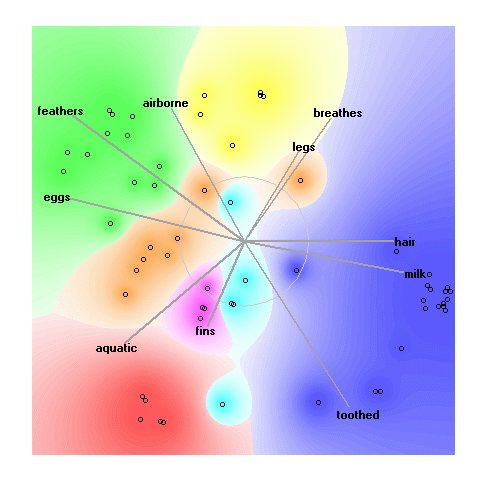
\includegraphics[width=12cm]{slike/zoo-freeviz.png}

\includegraphics[width=12cm]{slike/zoo-legenda.png}
\caption{Projekcija FreeViz iz podatkov o živalih}
\label{f-zoo-freeviz}
\end{center}
\end{figure}


Rezultat takšne projekcije na podatkih o živalih vidimo na sliki~\ref{f-zoo-freeviz}. Iz nje lahko, če znamo, razberemo veliko lastnosti podatkov. Na sliki so različna področja obarvana glede na prevladujočo živalsko vrsto - sesalci so modri, ribe rdeče in tako naprej. Osi ustrezajo atributom; smer osi nakazuje regijo, živalsko vrsto, ki jo sugerira visoka vrednost tega atributa. Vsi atributi, razen števila nog, so binarni, torej v tem primeru recimo dlake in zobje kažejo, da je žival verjetno sesalec. Iz osi torej razberemo povezavo med atributi in razredi, vidimo, katera živalska vrsta je značilna za posamezno lastnost, oziroma, katere lastnosti so značilne za posamezno živalsko vrsto.

FreeViz lahko beremo -- podobno kot MDS -- kot zemljevid. Ptiči in žuželke so si med seboj podobne; oboji letijo, zato v njuno smer kaže atribut {\em airborne}. Prav tako so si podobne ribe in dvoživke.

Vidimo lahko tudi podobnosti med atributi: kosmate živali dajejo mleko; živali, ki letajo, imajo perje, živali, ki plavajo, plavuti in živali, ki dihajo, noge. Obenem razberemo tudi glavne osi, po katerih lahko ločimo živali: žival bodisi daje mleko, bodisi vali jajca (vodoravna os) in je vodna žival s plavutmi ali pa dihajoča žival z nogami.

Osi, ki predstavljajo atribute, so različno dolge; čim pomembnejši je atribut, tem daljša je pripadajoča os. Manj pomembni atributi, katerih osi bi bile krajše od kroga v sredini, zaradi preglednosti niso narisani.

Končno, FreeViz je mogoče uporabljati tudi za uvrščanje primerov. Nov primer, katerega vrednosti atributov poznamo, razreda pa ne, lahko projeciramo in preverimo, v katero regijo je padel. Če v modro, je najbrž sesalec, če v zeleno, ptič\ldots

Ob uporabi FreeViza se moramo zavedati, da gre le za projekcijo v dvodimenzionalni prostor. Vse, kar vidimo, ni nujno resnično. Določeni atributi so morda tam, kjer so, samo zato, ker nekje pač morajo biti. Če uporabljamo FreeViz za iskanje vzorcev, moramo z njim dobljene vzorce preveriti, po možnosti na povsem novih podatkih ali pa jih primerjati z ekspertnim predznanjem o problemu.

FreeViza ne smemo uporabiti, kadar je število atributov primerljivo številu primerov ali celo večje. V tem primeru je mogoče kar analitično poiskati neskočno število rešitev, pri katerih so vse sile enake 0, razpored točk pa je v tem primeru nesmiseln. Slabost FreeViza je tudi, da v osnovi temelji na gradientni metodi in postane pri velikem številu točk počasen. Na lokalne ekstreme pa je, kakor je videti, dokaj neobčutljiv.


\cleardoublepage


\endinput

\section{Singularni razcep}

Oglejmo si podatke šestih filmskih zanesenjakov in njihovih ocenah filmov v tabeli~\ref{t:romance-sf}. Že na prvi pogled lahko opazimo, da imam najbrž dve skupini ocenjevalcev in dve skupini filmov. Metka, Neža, Maja in Tina ne marajo znanstvene fantastike in jim je bolj blizu romantika. Alojz in Gašper pa rajši gledata znanstveno fantastiko in jima romantični filmi niso prav blizu.

\begin{table}
\begin{tabular}{rcccccc}
\toprule
 & Cvetje & Titanic & Harry & Sally & Alien & Prometheus \\
\midrule
Metka & 1 & 2 & 1 & 0 & 0 \\
Neža & 2 & 4 & 2 & 0 & 0 \\
Maja & 3 & 5 & 3 & 0 & 0 \\
Tina & 5 & 10 & 5 & 0 & 0 \\
Alojz & 0 & 1 & 0 & 1 & 2 \\
Gašper & 0 & 0 & 0 & 2 & 4 \\
\bottomrule
\end{tabular}
\label{t:romance-sf}
\end{table}

Skupine pa nismo našli samo pri ocenjevalcih. Že zgoraj smo filme razvrstili v dve skupini, in te uganili iz kratkih nazivov filmov. Pa lahko te skupine, torej skupine uporabnikov in skupine filmov, razpoznamo algoritmično? Lahko podatke, ki jih imamo zgoraj, predstavimo v neki zgoščeni obliki, kjer bi iz zgoščenega zapisa bilo možno prepoznati skupine in interakcijo med ocenjevalci in filmi. Opazimo, recimo, da vsaka od vrstic v naši ocenjevalni tabeli izvira od enega od spodnjih vrstičnih vektorjev, ki ga moramo ustrezno pomnožiti z neko konstanto. 
% 
$$
\begin{bmatrix}
1 & 1 & 1 & 0 & 0 \\
0 & 0 & 0 & 1 & 1 \\
\end{bmatrix}
$$
Lahko take vektorje prepoznamo iz podatkov? Tehnika, ki jo bomo za to uporabili, se imenuje {\em singularni razcep}. Podatki iz tabele~\ref{t:romance-sf} so že sicer zapisani v atributni obliki in jih lahko torej predstavimo v matriki $A=\mathbb{R}^{m\times n}$. To matriko v splošnem s singularnim razcepom zapišemo kot produkt treh matrik:
\begin{equation}
A = U\Sigma V^\tr
\end{equation}
kjer so:
\begin{itemize}
\item leva singularna matrika $U\\mathbb{R}^{m\times r}$, ki $m$ objektov v vrsticah predstavi v $r$-dimenzionalnem prostoru,
\item desna singularna matrika 
\end{itemize}

